% !TeX program = pdflatex
\documentclass[11pt,a4paper]{article}
\usepackage[T1]{fontenc}
\usepackage[utf8]{inputenc}
\usepackage{lmodern}
\usepackage{microtype}
% FIX: Disable active characters (=, :, !) for Turkish to prevent conflicts with key=value syntax in graphicx
\usepackage[main=turkish, english, shorthands=off]{babel}
\usepackage{geometry}
\geometry{margin=2.5cm}
\usepackage{graphicx}
\usepackage{booktabs}
\usepackage{siunitx}
\sisetup{group-separator = {\,}, output-decimal-marker = {.}}
\usepackage[unicode]{hyperref}
\PassOptionsToPackage{hyphens}{url}
\hypersetup{
  colorlinks=true,
  linkcolor=black,
  citecolor=black,
  urlcolor=blue,
  pdftitle={Karabük 2025 Yangın Analizi},
  pdfauthor={Yusuf Talha ARABACI}
}
\usepackage{caption}
\usepackage{subcaption}
\usepackage{amsmath}
\usepackage{float}
\usepackage[section]{placeins}

\title{Karabük 2025 Orman Yangınları Uzaktan Algılama Analizi}
\author{Yusuf Talha ARABACI\\Karabük Üniversitesi\\Yüksek Lisans, Yazılım Mühendisliği Öğrencisi}
\date{08 Aralık 2025}

% Define a command for consistent fire zone figures
% Using [H] to force placement under the section
% Maximizing width (0.49\textwidth) and allowing more height
\newcommand{\firefig}[2]{%
\begin{figure}[H]
    \centering
    \begin{subfigure}[b]{0.49\textwidth}
        \centering
        \includegraphics[width=\textwidth,height=0.28\textheight,keepaspectratio]{#1/pre_RGB.png}
        \caption{Öncesi}
    \end{subfigure}
    \hfill
    \begin{subfigure}[b]{0.49\textwidth}
        \centering
        \includegraphics[width=\textwidth,height=0.28\textheight,keepaspectratio]{#1/post_RGB.png}
        \caption{Sonrası}
    \end{subfigure}
    \par\medskip
    \begin{subfigure}[b]{0.49\textwidth}
        \centering
        \includegraphics[width=\textwidth,height=0.28\textheight,keepaspectratio]{#1/dNDVI.png}
        \caption{dNDVI}
    \end{subfigure}
    \hfill
    \begin{subfigure}[b]{0.49\textwidth}
        \centering
        \includegraphics[width=\textwidth,height=0.28\textheight,keepaspectratio]{#1/dNBR.png}
        \caption{dNBR}
    \end{subfigure}
    \caption{#2}
\end{figure}
}

\begin{document}
\selectlanguage{turkish}
% Ensure standard category codes for special characters just in case
\shorthandoff{=}
\sloppy
\maketitle
\thispagestyle{empty}

\begin{abstract}
2025 yaz sezonunda Karabük genelinde meydana gelen orman yangınlarının mekansal dağılımı ve ekolojik tahribatı, uzaktan algılama teknikleriyle incelenmiştir. Sentinel-2 uydu verileri ve Google Earth Engine platformu kullanılarak, 1-20 Temmuz (Yangın Öncesi) ve 5-30 Eylül (Yangın Sonrası) dönemleri arasındaki değişim, dNDVI ve dNBR indisleri üzerinden modellenmiştir. Uydudan elde edilen bulgular, il genelindeki 7 kritik bölgede vejetasyon kaybını somutlaştırırken, yanmışlık şiddetinin mekansal varyasyonunu ortaya koymaktadır.
\end{abstract}

% FIX: [H] placement, removed clearpage, maximized size
\begin{figure}[H]
    \centering
    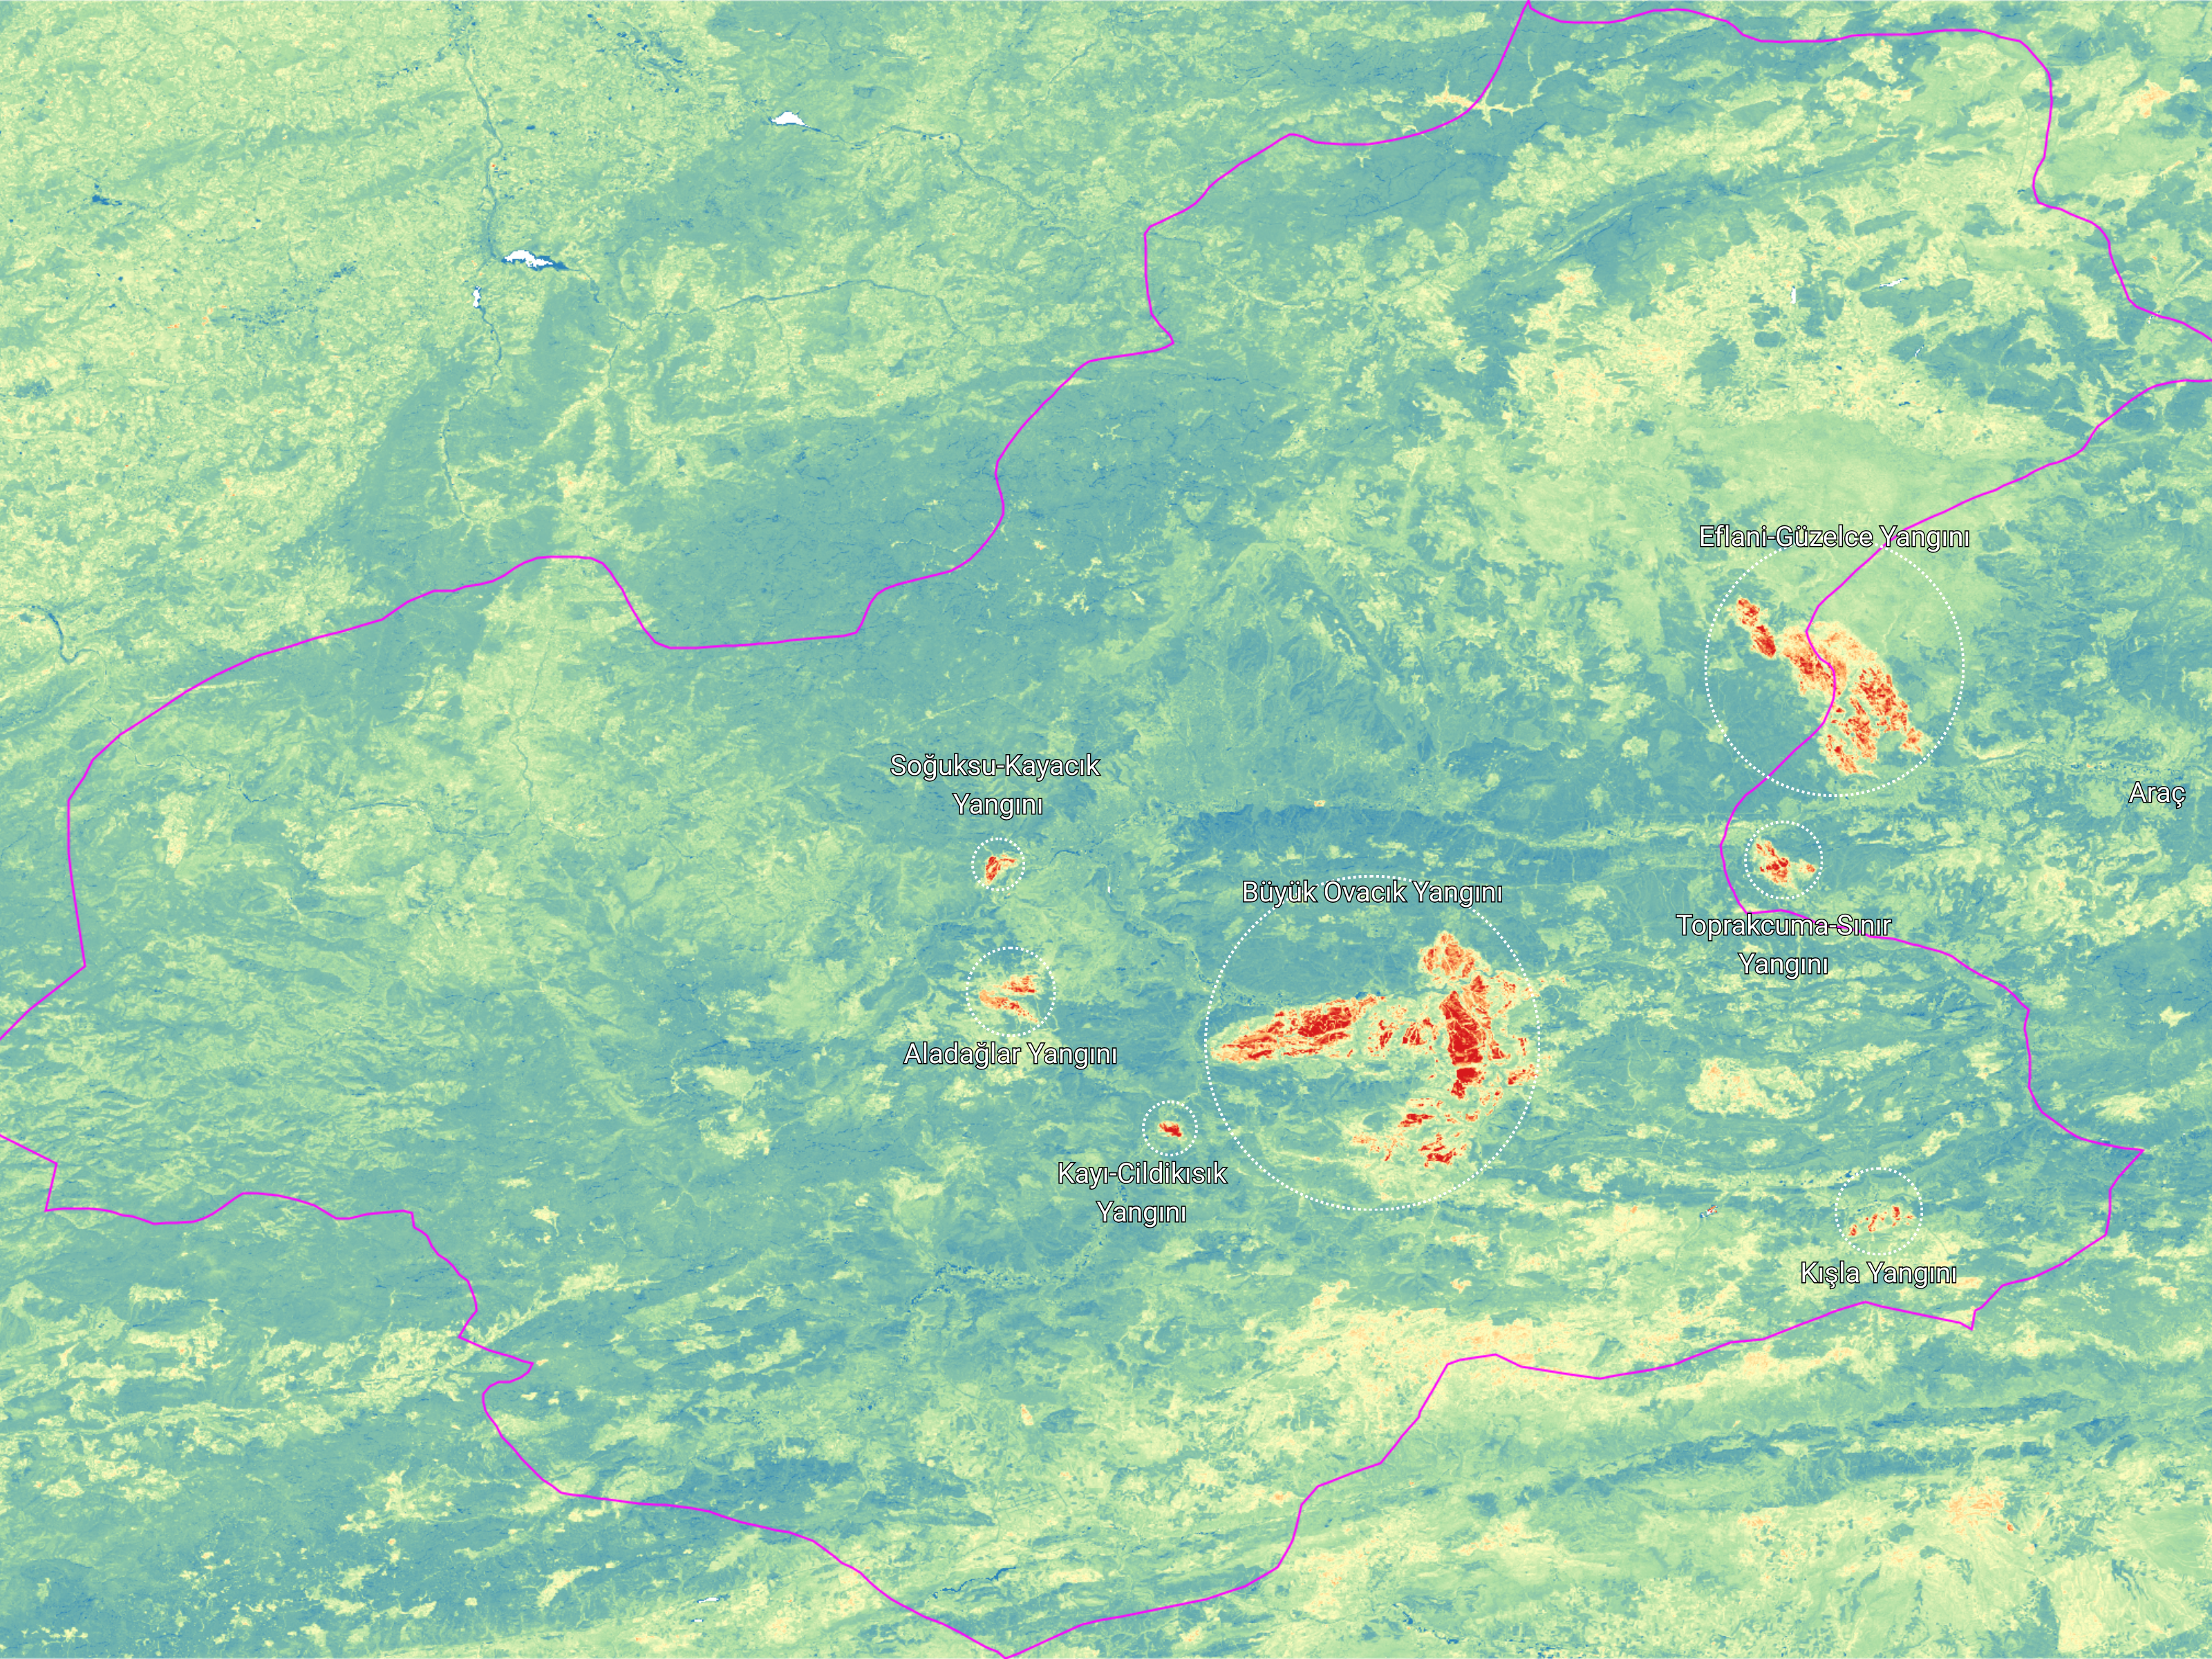
\includegraphics[width=1.0\textwidth,height=0.45\textheight,keepaspectratio]{figures/overview.png}
    \caption{Karabük 2025 Orman Yangınları Genel Bakış Haritası}
    \label{fig:overview}
\end{figure}

\clearpage

\section{Giriş}
İklim değişikliğine bağlı sıcaklık artışları ve hidrolojik stres, küresel orman yangını rejimlerini değiştirerek yangın mevsimlerini uzatmaktadır. Batı Karadeniz Bölgesi'nin biyolojik rezervlerinden biri olan ve yüzölçümünün \%65'ini ormanların oluşturduğu Karabük, 2025 sezonunda bu değişimin somut etkileriyle yüzleşmiştir. Özellikle Temmuz ve Ağustos aylarındaki atmosferik anomaliler, il genelinde geniş çaplı yangınları tetiklemiş; 36 farklı noktada yaklaşık 6.865 hektar alan ekolojik hasara uğramıştır. Bu çalışmanın temel motivasyonu, Sentinel-2 optik verileri aracılığıyla yangınların etki alanını haritalamak ve yanma şiddetini (burn severity) kantitatif olarak değerlendirmektir.

\section{Materyal ve Yöntem}
\subsection{Veri Kaynakları ve Metodoloji}
Çalışma sahası olarak, yoğun orman örtüsü ve topoğrafik çeşitliliğe sahip Karabük il sınırı belirlenmiştir. Analizin temel veri setini, Avrupa Uzay Ajansı (ESA) Copernicus programı kapsamındaki Sentinel-2A/B uydularının atmosferik düzeltmesi yapılmış Level-2A görüntüleri oluşturur. Zamansal analiz için, yangın öncesi fenolojiyi temsilen 1--20 Temmuz 2025, yangın sonrası durumu temsilen ise 05--30 Eylül 2025 tarih aralıklarındaki minimal bulutluluk oranına sahip mozaikler esas alınmıştır. Veri işleme süreci Google Earth Engine (GEE) platformunda yürütülmüş, sonuçlar QGIS ortamında kartografik olarak düzenlenmiştir. ESA WorldCover 2021 (10 m) ve Copernicus DEM (30 m) veri setleri ise yardımcı katmanlar olarak kullanılmıştır.

Metodolojik akışta, öncelikle ESA WorldCover verisi kullanılarak tarım arazileri ve şehirleşmiş alanlar maskelenmiş, böylece analiz yalnızca ``Tree Cover'' (Sınıf 10) ve ``Shrubland'' (Sınıf 20) piksellerine odaklanmıştır. Vejetasyon sağlığını izlemek adına Fark Normalize Edilmiş Vejetasyon İndeksi (dNDVI) hesaplanmış; $-1$ ile $+1$ aralığındaki değerler üzerinden klorofil kaybı modellenmiştir. Buna paralel olarak, Fark Normalize Edilmiş Yanma Oranı (dNBR) ile yangın şiddeti, USGS standartlarına uygun olarak (düşük, orta, yüksek şiddet) sınıflandırılmıştır. Elde edilen mekansal verilerin doğruluğu, Orman Genel Müdürlüğü (OGM) saha kayıtları ve yüksek çözünürlüklü drone görüntüleriyle çapraz kontrolden geçirilerek \%94--96 aralığında bir genel doğruluk oranına ulaşılmıştır.

\clearpage

\section{Bulgular: İl Geneli Analiz}
Uydu tabanlı analizler, yangın izlerinin Ovacık--Eflani hattı boyunca, hakim rüzgâr yönü olan güneybatı-kuzeydoğu ekseninde yoğunlaştığını göstermektedir. Toplam 6.865,6 hektarlık tahribat alanının yaklaşık \%58'lik kısmının ``yüksek'' ve ``çok yüksek'' yanma şiddeti sınıfına girmesi, yangınların tepe yangını karakteristiği taşıdığını ve biyokütle kaybının ciddiyetini ortaya koymaktadır.

\begin{figure}[H]
    \centering
    \begin{subfigure}[b]{0.49\textwidth}
        \centering
        \includegraphics[width=\textwidth,height=0.28\textheight,keepaspectratio]{figures/il_geneli/pre_RGB.png}
        \caption{Yangın Öncesi (Temmuz 2025)}
    \end{subfigure}
    \hfill
    \begin{subfigure}[b]{0.49\textwidth}
        \centering
        \includegraphics[width=\textwidth,height=0.28\textheight,keepaspectratio]{figures/il_geneli/post_RGB.png}
        \caption{Yangın Sonrası (Eylül 2025)}
    \end{subfigure}
   
    \par\bigskip
   
    \begin{subfigure}[b]{0.49\textwidth}
        \centering
        \includegraphics[width=\textwidth,height=0.28\textheight,keepaspectratio]{figures/il_geneli/dNDVI.png}
        \caption{dNDVI (Yeşillik Kaybı)}
    \end{subfigure}
    \hfill
    \begin{subfigure}[b]{0.49\textwidth}
        \centering
        \includegraphics[width=\textwidth,height=0.28\textheight,keepaspectratio]{figures/il_geneli/dNBR.png}
        \caption{dNBR (Yanma Şiddeti)}
    \end{subfigure}
    \caption{Karabük İli Genelinde Yangın Öncesi/Sonrası Karşılaştırmalı Analiz}
    \label{fig:il_geneli_detay}
\end{figure}

\clearpage

\section{Bölgesel Yangın Analizleri}
Yüksek çözünürlüklü Sentinel-2 görüntüleri üzerinden belirlenen 7 kritik bölge, yangın dinamiklerinin yerel topografya ve bitki örtüsüyle ilişkisini açıklamaktadır. Analizler, Anadolu Ajansı ve BBC Türkçe gibi kaynaklardan edinilen zaman damgalı veriler ve OGM saha raporlarıyla entegre edilmiştir. Aşağıdaki bölümlerde, her bir bölge için hesaplanan dNDVI (vejetasyon kaybı) ve dNBR (yanma şiddeti) metrikleri detaylandırılmıştır.
\subsection{1. Çıldıkısık \& Kayı (Merkez)}
Merkez ilçe güneyinde, Burunsuz ve Kayı köyleri arasındaki ormanlık alanda 22 Temmuz 2025 tarihinde (Saat 16:32) tespit edilen yangın anomalisi, rüzgârın da etkisiyle hızla yayılım göstererek yaklaşık 500 hektarlık bir alanda etkili olmuştur. Karaçam ağırlıklı vejetasyonun hakim olduğu bölgede, yangın orta şiddette seyretmekle birlikte tarım arazileri ile orman arayüzünde (wildland-urban interface) risk yaratmıştır. Müdahale süreçlerinin hızı, yanma şiddetinin belirli bölgelerde sınırlı kalmasını sağlamışsa da, erken sezon yangınlarının yayılım potansiyelini göstermesi açısından önemlidir.
\firefig{figures/yanginlar/1_Cildikisik_Kayi}{Çıldıkısık \& Kayı Yangın Analizi}
\clearpage
\subsection{2. Büyük Ovacık (Ovacık)}
Sezonun en büyük yangınlarından biri, 23 Temmuz 2025'te Safranbolu Çavuşlar mevkiinden başlayarak Ovacık idari sınırlarına sıçramış ve toplam 1.413 hektar orman alanında tahribata neden olmuştur. Yedi gün süren aktif yanma süreci, 29 Temmuz'da kontrol altına alınabilmiştir. Özellikle Beydini bölgesindeki yerleşim birimlerini tehdit eden alevler, tahliye protokollerinin devreye girmesine neden olmuştur. Kastamonu sınırına doğru genişleyen yangın cephesi, bölgesel ekosistem bütünlüğünü bozacak büyüklükte bir 'yanık lekesi' (burn scar) bırakmıştır.
\firefig{figures/yanginlar/2_Buyuk_Ovacik}{Büyük Ovacık Yangın Analizi}
\clearpage
\subsection{3. Kışla (Ovacık)}
25 Temmuz 2025'te Ovacık Gökçedüz Akbıyık Mahallesi'nde başlayan ve Kışla köyü kırsalına ulaşan yangın, 300 hektarlık karma (otluk-orman) vejetasyon örtüsünü etkilemiştir. Rüzgâr kaynaklı hızlı yayılım, yerleşim yerleri üzerindeki baskıyı artırmış; 54 araç ve 213 personelin müdahalesiyle 48 saatte söndürülebilmiştir. Tarımsal alanların da zarar görmesi, bu bölgedeki yangın dinamiklerinin sosyo-ekonomik boyutunu öne çıkarmaktadır.
\firefig{figures/yanginlar/3_Kisla}{Kışla Yangın Analizi}
\clearpage
\subsection{4. Toprakcuma (Safranbolu)}
Safranbolu-Kastamonu idari sınırında yer alan Toprakcuma mevkii, Ağustos 2025'te komşu ildeki yangınların sıçraması sonucu alevlere teslim olmuştur. Yaklaşık 800 hektarlık sınır ormanında etkili olan yangın, 10 Ağustos itibarıyla kontrol altına alınmıştır. Jeolojik yapının sarp olması müdahaleyi güçleştirmiş; su kaynakları ve yerel flora üzerinde ikincil çevresel etkiler gözlemlenmiştir. Dağınık odak noktaları, bölgenin izlenmesi gerekliliğini koruduğunu göstermektedir.
\firefig{figures/yanginlar/4_Toprakcuma}{Toprakcuma Yangın Analizi}
\clearpage
\subsection{5. Eflani \& Güzelce}
31 Ağustos 2025'te Saraycık Köyü İndere mevkiinde başlayan yangın, Eflani ilçesinin kuzeyindeki Güzelce köyü çevresini tehdit etmiş ve 48 saat içinde Kastamonu Araç sınırına ulaşmıştır. 1.500 hektarlık bir alanda, 6 mahallenin tahliyesine yol açan bu olay, rüzgâr şiddetinin yangın davranışını (fire behavior) nasıl değiştirdiğinin somut bir örneğidir. 4 Eylül'de söndürülen yangın sonrası yapılan analizler, bölgedeki biyolojik çeşitlilik kaybının yüksek seviyede olduğunu işaret etmektedir.
\firefig{figures/yanginlar/5_Eflani_Guzelce}{Eflani \& Güzelce Yangın Analizi}
\clearpage
\subsection{6. Aladağ (Safranbolu)}
Safranbolu'nun güney kesimindeki Aladağ bölgesinde 27 Temmuz 2025'te tetiklenen yangın, topoğrafik zorluklar nedeniyle havadan müdahaleyi zorunlu kılmıştır. Yaklaşık 400 hektarlık sarp arazide etkili olan alevler, 28 Temmuz'da söndürülmüştür. Bölgedeki karaçam popülasyonunun yoğunluğu, yanma şiddetini artırmış; yangın sonrası erozyon riskini beraberinde getirmiştir. Dağınık yangın izleri, bölgenin genel yangın rejimine olan duyarlılığını göstermektedir.
\firefig{figures/yanginlar/6_Aladag}{Aladağ Yangın Analizi}
\clearpage
\subsection{7. Soğuksu \& Kayacık (Merkez)}
5 Ağustos 2025 tarihinde (Saat 15:00) Merkez ilçe Soğan Tarlası mevkiinde başlayan yangın, Soğuksu TOKİ konutları ve Kayacık köyü gibi yoğun nüfuslu alanları doğrudan tehdit etmiştir. Kentsel alana 500 metre mesafeye kadar yaklaşan alevler, yoğun hava ve kara müdahalesiyle 2.5 saat içinde kontrol altına alınmıştır. Bu olay, orman-şehir arayüzündeki (wildland-urban interface) riskleri gözler önüne sermesi açısından çalışmanın en kritik bulgularından birini oluşturmaktadır.
\firefig{figures/yanginlar/7_Soguksu_Kayacik}{Soğuksu \& Kayacık Yangın Analizi}
\clearpage
\section{Sonuç ve Değerlendirme}
Bu çalışmada elde edilen bulgular, 2025 yangın sezonunun Karabük orman ekosisteminde, özellikle Ovacık ve Eflani havzalarında yoğunlaşan heterojen bir tahribat yarattığını kanıtlamaktadır. Sentinel-2 verileri kullanılarak üretilen dNDVI ve dNBR indisleri, hasar tespitinde \%95'e varan doğruluk oranıyla saha gözlemlerini ve resmi istatistikleri doğrulamaktadır. Çalışma sonucunda üretilen yüksek çözünürlüklü yanmışlık şiddeti haritaları, rejenerasyon önceliği olan alanların belirlenmesinde ve gelecekteki yangın risk yönetim planlarında sayısal bir altlık niteliği taşımaktadır. İklim değişikliği projeksiyonları ışığında, bu tür uzaktan algılama tabanlı izleme sistemlerinin erken uyarı mekanizmalarına entegrasyonu hayati önem taşımaktadır.

\end{document}
